\section{Introduzione}

Lo scopo di questa esperienza di laboratorio è quello di montare un impianto da vuoto che risulti in
grado di raggiungere pressioni dell'ordine di $10^{-3}$ \si{\pascal}. Inoltre l'esperienza serve anche a
prendere dimestichezza con le varie componenti che costituiscono l'impianto da vuoto.
Infine l'ultimo obbiettivo, ad impianto funzionante, è quello di tarare un vacuometro Pirani.

\section{Materiale utilizzato}

Il materiale messo a nostra disposizione è il seguente:

\begin{itemize}
	\item{una camera con un volume di $5930 \pm 10$ \si{\centi\metre}$^3$;}
	\item{una pompa rotativa con pressione di vuoto limite dell'ordine di qualche Pascal;}
	\item{una pompa ibrida turbomolecolare-molecular drag con relativa elettronica;}
	\item{cravatte e O-ring in Viton di varie dimensioni;}
	\item{tubi e raccordi con flange;}
	\item{2 valvole a membrana, 1 valvola a perdita calibrata, 1 valvola gate;}
	\item{2 vacuometri Pirani, 1 vacuometro a ionizzazione a catodo caldo e 1 vacuometo a ionizzazione a catodo freddo;}
	\item{cavi e lettore AGC per i quattro sensori sopracitati;}
\end{itemize}

\section{Esecuzione dell'esperienza}

\subsection{Montaggio dell'impianto da vuoto}

Per quanto riguarda il montaggio dell'impianto da vuoto abbiamo utilizzato il materiale sopraelencato
prestando attenzione che fossero rispettate le richieste dei tecnici di laboratorio;
ovvero che l'impianto soddisfacesse i seguenti requisiti:

\begin{itemize}
	\item{si deve poter isolare la pompa turbomolecolare dal resto dell'impianto per proteggerla da sbalzi di pressione;}
	\item{si deve poter misurare la pressione nelle vicinanze della pompa turbomolecolare per tenerla sotto controllo ed evitare danni ad essa;}	
	\item{si deve poter portare la camera da vuoto dalla pressione atmosferica ad una pressione bassa e viceversa, senza spegnere la pompa turbomolecolare per non sprecare tempo;}
	\item{si deve poter misurare la pressione in camera con i diversi strumenti a nostra disposizione;}
\end{itemize}

Seguendo questi requisiti abbiamo realizzato uno schema su carta dell'impianto tenendo conto del materiale a nostra disposizione. Dopo aver realizzato lo schema, abbiamo montato l'impianto facendo attenzione ad associare ad ogni flangia il corretto O-ring e la corretta cravatta, fissando il tutto adeguatamente. Lo schema dell'impianto è riportato in Figura \ref{fig:schema}.

\subsection{Funzionamento dell'impianto da vuoto}
\paragraph{Creazione del prevuoto\\}
Il prevuoto, indispensabile per avviare la pompa turbomolecolare, è stato ottenuto semplicemente avviando la pompa rotativa, tenendo chiusa la sola valvola che collega direttamente la camera da vuoto e l'atmosfera.
\paragraph{Vuoto in camera\\}
Per creare il vuoto in camera è necessario prima creare il prevuoto con la pompa rotativa. Una volta raggiunte le condizioni adatte, cioé il sistema è ad una pressione dell'ordine di qualche \si{\Pa}, si chiude la valvola del bypass e si può accendere la pompa turbomolecolare. Infine basta lasciare lavorare il sistema affinché arrivi alla sua pressione limite o alla pressione desiderata.
\paragraph{Rientro di aria a pressione atmosferica in camera\\}
Dalla situazione di vuoto in camera, per effettuare il rientro di aria in camera, mantenendo accesa la pompa turbomolecolare, è necessario prima di tutto chiudere la valvola gate, in modo che la pompa turbomolecolare non si danneggi subendo una brusca variazione di pressione. Mantenendo chiusa la valvola del bypass occorre lasciare che la pompa rotativa aspiri il fondo della pompa turbomolecolare. Quindi basta aprire la valvola che collega la camera da vuoto con l'atmosfera ed effettuare il rientro d'aria in camera.
\paragraph{Ritorno ad una situazione di alto vuoto in camera.\\}
Per ritornare ad una bassa pressione in camera, dalla situazione descritta nel paragrafo precedente, è necessario chiudere la valvola a fondo della turbo per isolarla completamente. In seguito si deve aprire la valvola del bypass in modo tale da creare il prevuoto in camera con la pompa rotativa. Una volta che la pressione segnalata da entrambi i vacuometri Pirani è uguale, si può aprire la valvola a fondo della pompa turbomolecolare e chiudere la valvola del bypass. Le operazioni fin qui descritte vanno eseguite con una certa rapidità per evitare che a fondo della pompa turbomolecolare si crei una zona con pressione troppo elevata. L'ultima operazione è quella di aprire lentamente la valvola gate, in modo da non sforzare la pompa turbomolecolare, per poi lasciare che l'impianto raggiunga nuovamente la condizione di vuoto limite.
\paragraph{Vacuometri a catodo caldo e a catodo freddo\\}
Durante tutta l'esecuzione dell'esperienza si è prestata attenzione all'accensione e allo spegnimento di tali vacuometri onde evitare di provocare danni. Il vacuometro a catodo caldo infatti deve operare al di sotto dei $10^{-4}$ \si{\pascal} affinché non si bruci il filamento al suo interno. Il vacuometro a catodo freddo invece deve operare al di sotto dei $10^{-4}$ \si{\pascal} affinché non si ossidi la superficie interna.

\subsection{Taratura dei vacuometri Pirani}

Per tarare il vacuometro Pirani, che misurava la pressione in camera, abbiamo portato la pressione oltre il limite inferiore
della sensibilità dello strumento, specificato nel manuale. Il manuale riporta un range massimo di funzionamento che va da $10^{-2}$ \si{\pascal} fino a $10^5$ \si{\pascal}, anche se l'intervallo in cui la precisione è buona è tra 0.1 \si{\pascal} e $10^4$ \si{\pascal}. Abbiamo quindi impostato il voltaggio in uscita al valore di 2 Volt lavorando su un potenziometro. Dopo aver isolato la pompa turbomolecolare dal resto dell'impianto abbiamo riportato la pressione della camera alla pressione atmosferica. A questo punto si è impostato il valore di output del sensore a 10 Volt, lavorando su un secondo potenziometro. Infine abbiamo riportato la pressione in camera a bassa pressione per controllare che il voltaggio al limite inferiore fosse ancora 2 Volt. Può succedere infatti che la regolazione del secondo potenziometro renda vana la prima regolazione.

\subsection{Qualche dato}

La pressione in camera ottenuta grazie al solo utilizzo della pompa rotativa è stata di circa:

\begin{equation}
    P \,=\, 1.8  \; \si{\pascal}
\end{equation}
%
La pressione limite da noi raggiunta, misurata con il vacuometro a catodo caldo, è di circa:

\begin{equation}
    P \,=\, 6.85 \cdot 10^{-4} \; \si{\pascal}
\end{equation}

\begin{figure}[b!]
    \centering
   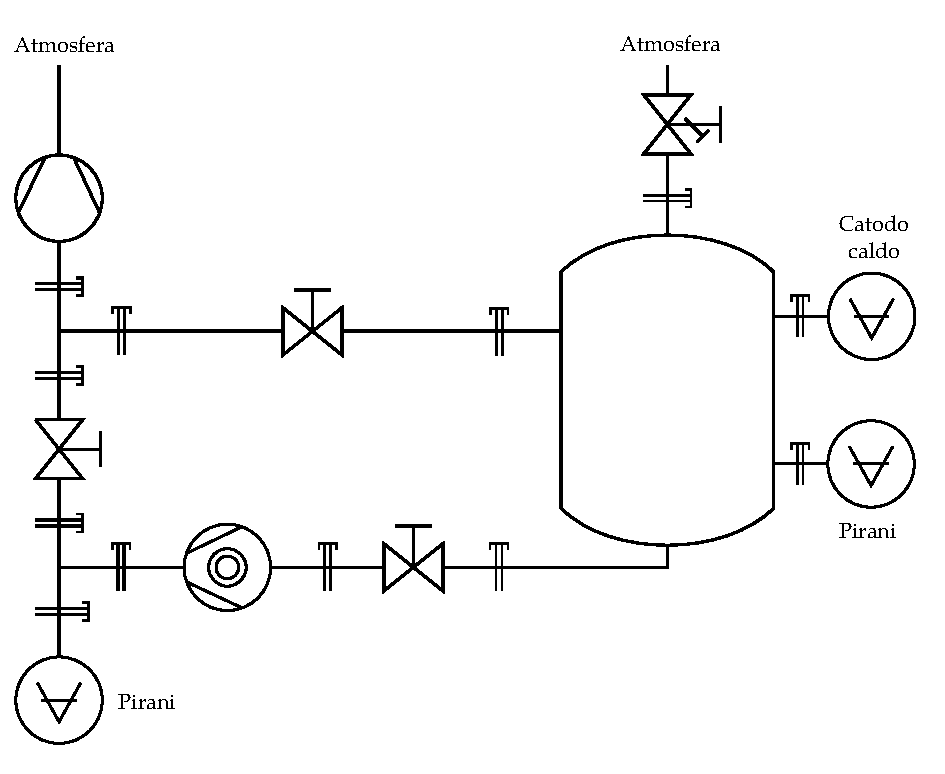
\includegraphics[width=16cm]{drawing.pdf}
   \caption{Schema dell'impianto da noi realizzato. La pompa primaria è una pompa rotativa, mentre la seconda pompa al centro dello schema
   è una pompa turbomolecolare. Sono visibili il bypass e i tre diversi sensori di pressione collegati alla camera da vuoto. La pompa
   turbomolecolare poteva essere isolata dal resto dell'impianto grazie alla valvola gate e alla valvola sul fondo della pompa.}
   \label{fig:schema}
\end{figure}